\documentclass{article}
\usepackage{../fasy-hw}

%% UPDATE these variables:
\renewcommand{\hwnum}{2}
\title{Discrete Structures, Homework 1}
\author{Patrick O'Connor (Patrick OConnor (322))}
\collab{n/a}
\date{due: 5 February 2021}

\begin{document}

\maketitle

This homework assignment should be
submitted as a single PDF file both to D2L and to Gradescope.

General homework expectations:
\begin{itemize}
    \item Homework should be typeset using LaTex.
    \item Answers should be in complete sentences and proofread.
    \item You will not plagiarize.  \item List collaborators at the start of
    each question using the \texttt{collab} command.
    \item Put your answers where the \texttt{todo} command currently is (and
        remove the \texttt{todo}, but not the word \texttt{Answer}).
\end{itemize}

% ============================================
% ============================================
\collab{Liam,Dustin,Robert Van Spyk} \nextprob{Everyday Mathematical Arguments}
% ============================================
% ============================================
Your sister and you decided to partner on a car washing endeavor, where you
charge cars $\$10$ for a car wash and to split the earnings.  Since you are
doing this at your parents house and they had extra soap, sponges, and a hose
available, there are no costs to you.  At the end of the first day, you have
earned $\$45$ and she had only earned $\$10$. She claimed that you did not pay
her the full payment she deserved. Her argument was: ``If we wash a car, you
earn $\$5$ and I earn $\$5$.  If you earned $\$45$, then we washed nine cars.
Ifwe wash nine cars, I have earned $\$45$.  I have earned $\$10$; therefore, you
did not give me all of the money that I earned.''  Now, she has not yet taken
Prof.~Fasy's Discrete Structures class, so she does not see the fallacy in her
argument. First, explain which statement that she made that she could not
correctly conclude and explain why.  Second, counter her argument, using
everyday English. The last sentence of your argument should be ``Therefore, I
earned $\$45$ and you earned $\$10$. Third, write this counter argument using
logic statements by first listing the logic statements then writing the argument
mathematically.  Be sure to explain which arguments from Table 2.3.1 that you
are using.

\paragraph{Answer}

My sister made a converse error in that she assumed that because I earned $\$45$
during the day of being at the washing spot we washed a total of nine cars.
We in fact only washed 2 cars at $\$10$ a car for a total of
$\$20$ divided by 2 for $\$10$ each. On top of our agreement I wash a total of 7 bikes
from the local muddy children. A bicycle wash at my house is $\$5$ and with this
I made $\$35$ plus the $\$10$ from cars for a total of $\$45$ while she only got $\$10$
from the car wash. Therefore, I earned $\$45$ and She earned $\$10$ from day 1.

Consider the following statements:
\begin{enumerate}
    \item p = We washed nine cars
    \item q = You earned $\$45$
    \item r = Converse error if p then q.

If q then p is a converse error as q does not necessarily imply p
\end{enumerate}



% ============================================
% ============================================
\collab{Liam,Dustin,Robert Van Spyk}
\nextprob{Existential Statements}
% ============================================
% ============================================

Are the following statements true or not true?    Prove or disprove.

\begin{enumerate}

    \item All even integers are equal to an odd integer plus one.

        \paragraph{Answer}
        If one is added to an even integer a it is now a+1 = b
        By definition an odd number is (even number + 1) and
        b is an even number a+1
        Therefore, all even integers are equal to an odd integer plus one.

    \item All horses are the same color.

        \paragraph{Answer}
        If all horses are the same color, then no to horses have
        differing colors.
        There are two horses with different colors.
        Therefore not all horses are the same color.

\end{enumerate}


% ============================================
% ============================================
\collab{N/A}
\nextprob{Division into Cases}
% ============================================
% ============================================

When working at Lockheed Martin, I was invited to play Texas
Hold'em\footnote{For rules, see
here:\url{https://www.pokernews.com/poker-rules/texas-holdem.htm}} at my
colleague's house.  I play with the following rules:
\begin{itemize}
    \item Never fold before the flop.
    \item Never increase the bet.
    \item If it is possible that my hand is \emph{three of a kind} or better,
        match the bet.  Otherwise, fold.
\end{itemize}
My current hand is the jack of hearts and the 10 of diamonds, and the flop is 10
of hearts, 3 of clubs, and king of hearts.

\begin{enumerate}

    \item What are the cases that could occur for the Turn card?  What is the
        outcome (match or fold) for these different cases? (Note: rather than
        listing every possible card, try to categorize the cards into as few
        classes as possible).

    \paragraph{Answer}
    Having a current hand of the jack of hearts and the 10 of diamonds, and a
    flop of 10 of hearts, 3 of clubs, and king of hearts. The possible cases
    that could occur for the Turn card ranking from best to worst are 3 of a
    kind(10's), Two pair of (existing 10's pair and turn of another(J, 3, or K))
    , One pair, or High card. The Two pair(10's pair and turn of
    another(J's, 3's, or K's)), One pair, and High card are all not
    sufficient in satisfying condition number 3 noted above and would
    result in fold. Although the majority of your options are not sufficient,
     the three 10's would result in matching the bet and it is still a
     possibility so match and go into River round.

    \item Suppose that the Turn card is the jack of clubs.
        What are the cases that could occur for the River card, and what is the
        outcome (match or fold) for these different cases?  (Again, try to
        describe this in as few cases as possible).

    \paragraph{Answer}
    Having a current hand of the jack of hearts and the 10 of diamonds, a
    flop of 10
    of hearts, 3 of clubs, and king of hearts and turn of jack of clubs.
    The possible cases that could occur for the River card
    ranking from best to worst are Full House(Deal J or 10 resulting in 3
    of a kind and use the other as the pair), 3 of a kind(10's or J's),
    Two pair of (existing 10's/J's pair or turn of another(3, or K)), One
    pair, or High card. The Two pair(10's/J's pair and dealing of
    another(3's, or K's)), One pair, and High card are all not
    sufficient in satisfying condition number 3 noted above and would
    result in fold. Although the majority of your options are not sufficient,
    Full House(Deal J or 10 resulting in 3 of a kind and use the
    other as the pair) or 3 of a kind(10's or J's) would result in matching
    the bet and it is still a possibility so match and go into Showdown.

\end{enumerate}


% ============================================
% ============================================
\collab{N/A}
\nextprob{Bipartite Graphs}
% ============================================
% ============================================

Exercise Set 4.9, Question 23.
\begin{figure}
  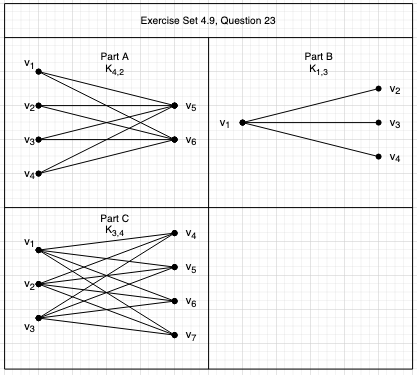
\includegraphics[width=\linewidth]{/question23.png}
  \caption{Graph for question 23 (a,b,c)}
  \label{fig:question23}
\end{figure}

\paragraph{Answer}
Part d) How many vertices of K$_{m,n}$ have a degree m? degree n?
If n not equal to m, the vertices K$_{m,n}$ are divided into two groups of size (n and m).
Every vertex in the group of size m has degree n because each is connected to
every vertex of size n. So K$_{m,n}$ has m vertices of degree n.
Similarly the same is true for group n in that every vertex in the group of
size n has degree n because each is connected to every vertex of size m.
In conclusion K$_{m,n}$ has n vertices of degree m.
If n=m then all of n+m = 2n vertices have the degree n.


Part e) What is the total degree of K$_{m,n}$?
The total degree of K$_{m,n}$ is m+n.


Part f) Find the formula in terms of m and n for the number of edges of K$_{m,n}$?

The formula for find the number of edges of K$_{m,n}$ is (mn)=edges.
This can be justified in that
each vertex of size n is connected to each vertex of size m.


% ============================================
% ============================================
\collab{N/A}
\nextprob{Four Color Theorem}
% ============================================
% ============================================
Read Chapter 1 of \emph{Four Colors Suffice} and answer the following questions:

\begin{enumerate}

    \item Consider the map of the continental US on Page 5.  Why can we color
        Utah and New Mexico the same color, even though the two states touch at
        a point?

        \paragraph{Answer}
        It is a convention of the Four Color theorem that if the touching
        section is a point, the two "countries", in this case Utah and
        New Mexico, are allowed to be the same color.

    \item Again, looking at the map of the continental US on Page 5, explain why
        Michigan does not satisfy the conditions for the four color theorem.

        \paragraph{Answer}
        The current version discussed in the book would cause Michigan to
        not satisfy the four color theorem as Michigan is split between
        two different "countries".
        It is a requirement of this theorem that a country must be in one piece.

    \item Explain why we an omit the states of Hawaii and Alaska in order to
        construct a four-coloring of the states in the USA.

        \paragraph{Answer}
        We can omit the states Hawaii and Alaska as they are not attached
        to any point of the 48 other states.

    \item Is the following statement TRUE or FALSE?  Explain. Four colors are
        necessary to color all maps.

        \paragraph{Answer}
      False, four colors are not necessary to color all maps. There are
      some maps that only need 3 colors such as the map below.
      \begin{figure}
        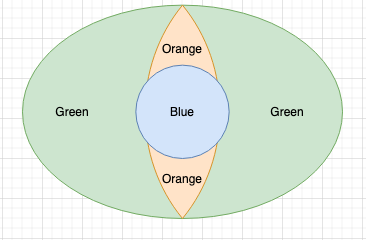
\includegraphics[width=\linewidth]{/3-color-map.png}
        \caption{Only 3 colors needed following the four color theorem}
        \label{fig:3ColorMap}
      \end{figure}


    \item Explain one application of the four color theorem that does not
        involve coloring geographic maps.

        \paragraph{Answer}
        An application of the four color theorem that is not coloring geographic maps is the delivery of signal(radio-frequency) to your devices.
        In order to decrease interference, using different frequencies is essential to avoid confusion.
        Using the cell towers and there effective signal range a node and edge graph can be create.
        With the four color thereom you can determine what frequencies should be assigned to which towers based on coloring in signal radius.
        Therefore using the least amount of differing frequencies, the overall cost of distribution is decreased.

    \item (Extra Credit). Provide a four-coloring of the McGregor April Fool's
        Hoax on Page 11.

        \paragraph{Answer}
        In the below figure it can be seen that it is possible to color the 110 region map with only 4 colors.
        \begin{figure}
          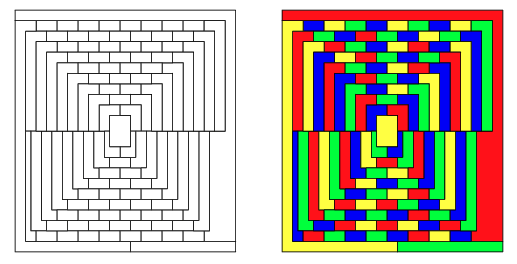
\includegraphics[width=\linewidth]{/mcgregorMap.png}
          \caption{April Fool's Joke done correctly to the four color thereom}
          \label{fig:McGregorMap}
        \end{figure}

\end{enumerate}

% ============================================
% ============================================
\collab{N/A}
\nextprob{Fred Brooks}
% ============================================
% ============================================

Write a short (1-2 paragraph) biography of Fred Brooks.  He wrote the book
entitled \emph{The Mythical Man Month}~\cite{brooks-manmonth}.  In your
biography, explain what the title of this book means.
\textbf{In your own words}, describe who they are and why they are important in
the history of computer science.  If you use external resources, please provide
proper citations. If you do not use external sources, please write ``I did not
use any sources to write this biography'' as the last sentence of the
biography.

\paragraph{Answer}

Frederick Phillips Brooks, Jr. was an American computer scientist from North Carolina. Brooks started his scientific career
with a degree in physics from Duke University and shortly after finishing his bachelors he proceeded to graduate from Harvard in applied mathematics.
After studying under Howard Aiken a computer pioneer, he joined IBM to work on the IBM 7030. The IBM 7030 was a super computer ordered by US National Security Agency.
Once completed Brooks continued his work in IBM by managing the IBM OS/360 operating system and its associated computers. During this project he was responsible in
selecting the 8-bit byte as the basic unit and included a complete set of alphanumerical characters. This decision made by him has transformed and is in almost every computer
used today in 2021. After an overall successful career in the private sector, Brooks decided to give back and dedicate the remaining years to education,
research and board participation. Brooks started his academic profession at UNC-Chapel Hill in which there was not a computer science department in existence yet.
Starting a now respected department with a focus on research expenditures in human-computer interaction, three-dimensional computer graphics and virtual reality.
Within the virtual reality realm, he lead the creation of scientific visualization tools that compounded to solving the physical structure of new protein molecules.

With an abundance of experience comes wisdom for most people and Brooks is not an exception. With this wisdom he decided to write and publish the
book titled "The Mythical Man Month" as a way of expressing his distain to the common ideology of adding more humans to a project that is running late
will speed up the timeline. This ideology is applicable in certain fields but complex software development is not one of them as with more programmers comes the time
taken from working to catch newbies up, increased communication overhead. These two extremely time consuming task will do quite the opposite of speeding things up and most likely
will end up delaying deployment even further.



%% ... the bibliography
\newpage
\bibliographystyle{acm}
\bibliography{biblio}

My bibliography wont work currently I have is above in figure. Any suggestions are greatly appreciated. Thank you.
\begin{figure}
  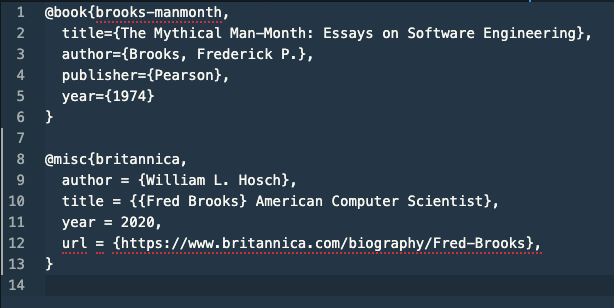
\includegraphics[width=\linewidth]{/bibProblems.png}
  \caption{Screenshot from my .bib file}
  \label{fig:bibProblems}
\end{figure}

Figure \ref{fig:question23} Exercise Set 4.9, Question 23 Part a,b, \newline
Figure \ref{fig:3ColorMap} shows a map done properly with only 3 colors \newline
Figure \ref{fig:McGregorMap} shows properly done McGregor Map \newline
Figure \ref{fig:bibProblems} Screenshot from my .bib file that isnt working


\end{document}
